%!TEX root = main.tex

\chapter{Implementation}
In this chapter we describe how we implemented the project.
Section \ref{sec:overview} we explain why we did what we did.
Section \ref{sec:integration} how we integrated bwapi with lida
Section \ref{sec:detectors} feature detectors we made
Section \ref{sec:actionexecution} how action are executed from lida to bwapi

\section{Overview} 
\label{sec:overview}
We chose the LIDA framework to work with both because it has a strong theoretical underpinning, and also because it is is easily available and is well-documented and has an active community working with and on it.

We also chose to ``cheat'' in our implementation by enabling perfect information in BWAPI, so we wouldn't need to implement behaviour for scouting yet.

\section{Integration}
\label{sec:integration}
BWAPI itself provides only a basic C++ API, so JNIBWAPI provides, as explained in chapter \ref{sec:starcrafttheory}, a custom Java API using the Java Native Interface, JNI.\cite{jni} But because we can't load an entire Java VM into the StarCraft process, we use shared memory to connect the StarCraft process with the process of our agent. We found that to do this you need to run the processes with Administrator privileges in Windows.

We also updated JNIBWAPI to adapt to some minor recent changes in BWAPI, and added in some missing functionality that we needed for controlling the game, like starting, pausing and restarting the on-going game.

But to use the LIDA framework this has to be integrated with JNIBWAPI. So to accomplish this we implement the domain specific modules of the LIDA framework to make calls to JNIBWAPI. 


\begin{figure}[h!tb]
\centering
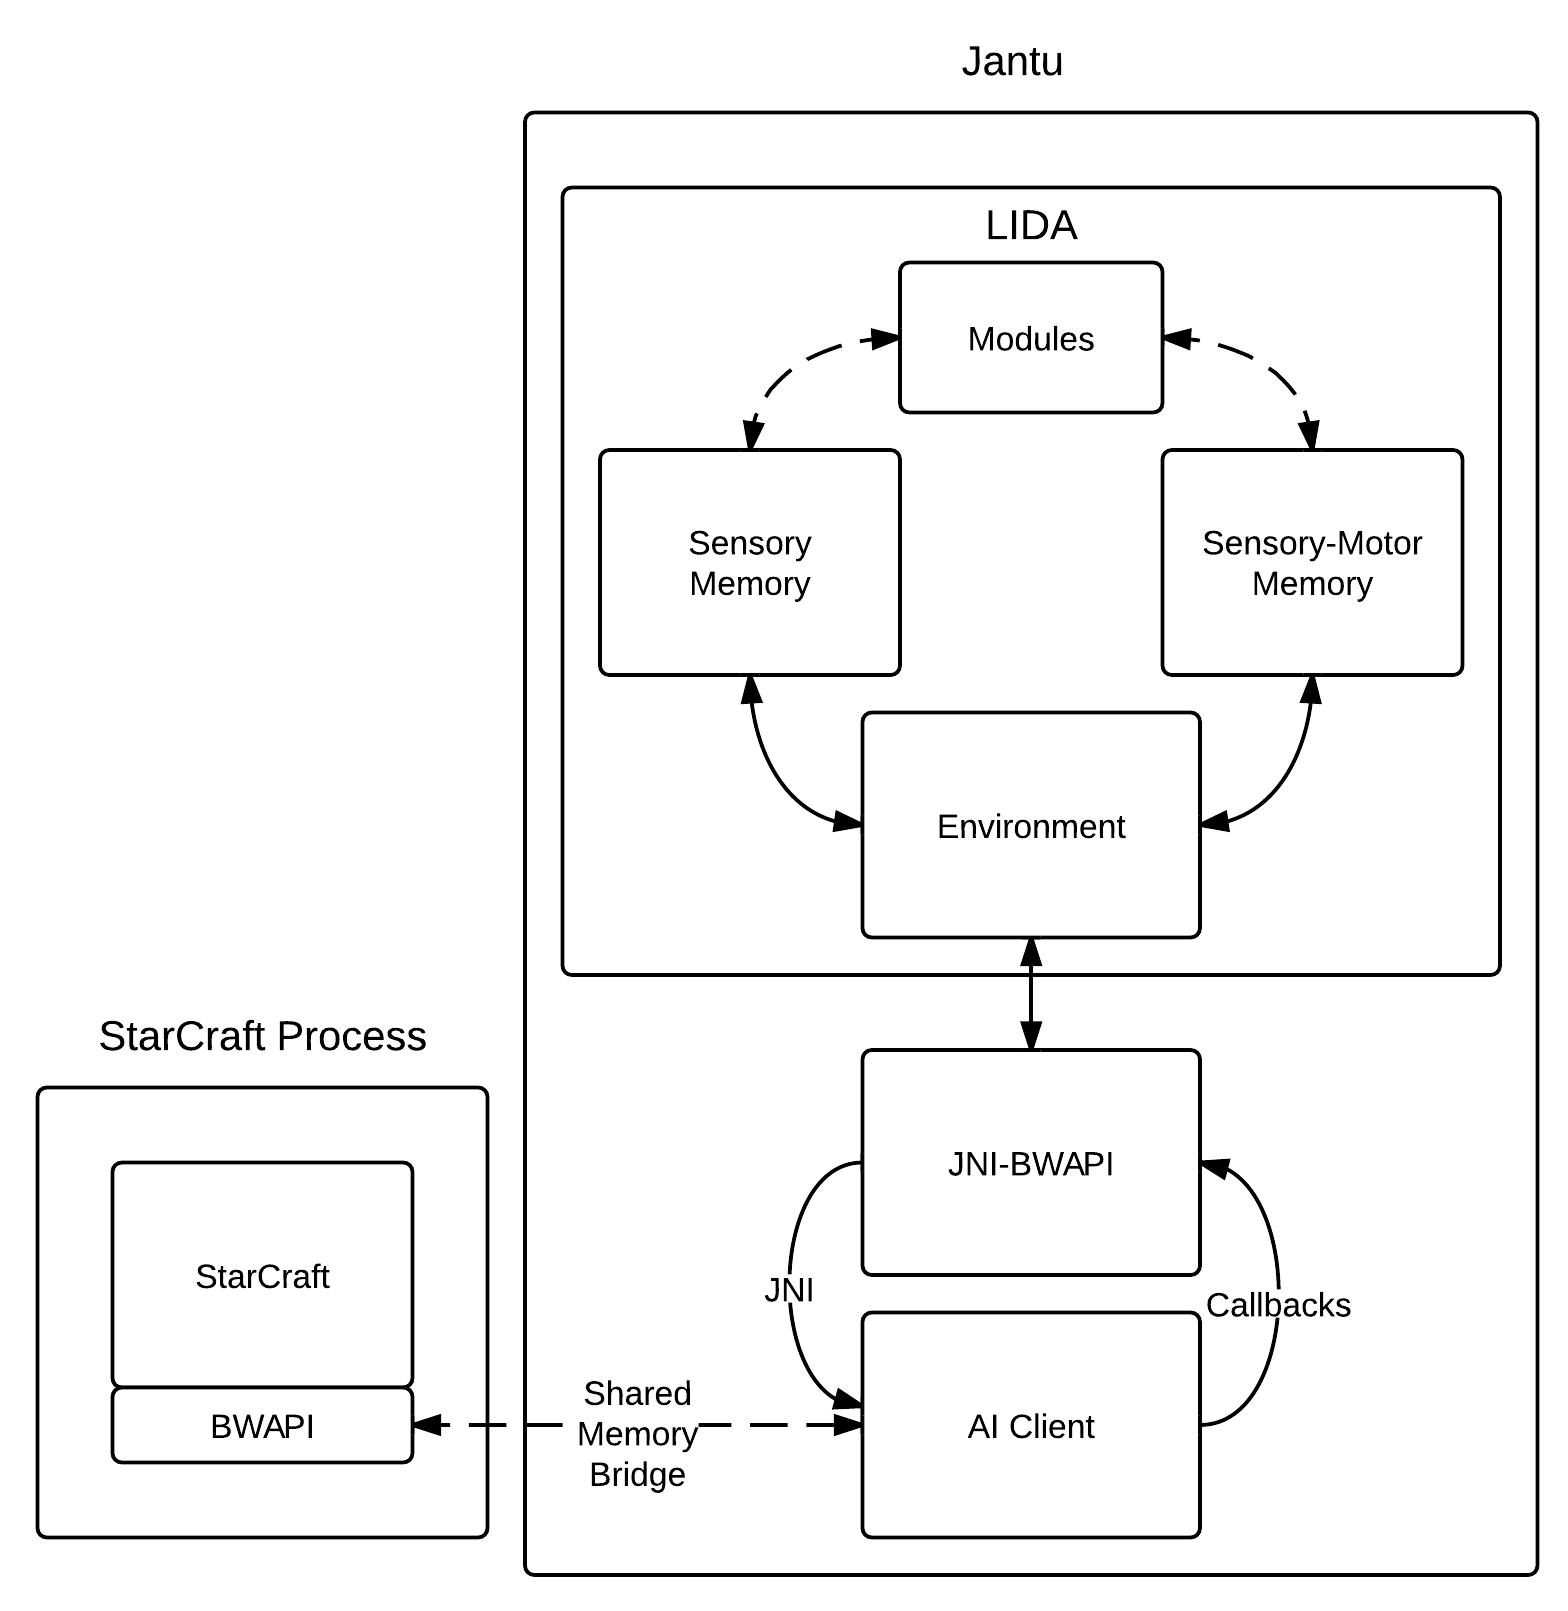
\includegraphics[scale=1.0]{graphics/jantu.png}
\caption{A general architecture overview of Jantu}
\label{fig:jantu}
\end{figure}

Figure \ref{fig:jantu} shows a general overview of the Jantu bots architecture, which consists of 3 main parts. In the Starcraft process the game it self runs together with BWAPI injected into the game client. Since this is all running in c++ and we are using the Java interface for BWAPI our code is run in a separate process that communicates with the Starcraft process using a shared memory bridge, this enables JNI-BWAPI to make calls to BWAPI and retrieve information back across the bridge. 

In the Jantu process JNI-BWAPI is running together with the LIDA framework. In order to integrate the LIDA framework with JNI-BWAPI we setup the framework first with the configurations we needed to get it up and running. This involves describing and structuring the modules you need in different XML configuration files. Also in these files we configure what kind of information that will be possible to use and transmit internally in the LIDA framework. 

JNI-BWAPI consists of different models and types that represent Starcraft information like units and buildings together with a lot of native functions that can be called to communicate with BWAPI. So we integraded this with LIDA by using a custom implementation of the Environment class in LIDA. This class becomes the interface between the domain specific modules of LIDA, the sensory memory and sensory-action memory, and JNI-BWAPI. 


\subsubsection{Environment module}
The Environment module is the interface between JNI-BWAPI and LIDA. It is responsible for abstracting away the JNI-BWAPI, and making sure that the game runs when it should. It allows LIDA to reset the state of the environment, by restarting the game.
\paragraph{Timing} When working with a congnitive architecture it is important to be able to look at the internal structures of the model during runtime, like the current situation model and what node structures have what activations. This is usefull for debugging and performance tweaking. To achive this we have to be able to pause and resume the game at anytime, so to the run/pause and timing functionality of LIDA inside StarCraft, we have a semaphore that is released by a LIDA codelet each tick. Then the callback from StarCraft/BWAPI waits for this to be released. This allows us to easily set the amount of StarCraft frames that are processed for each LIDA cycle, by increasing the amount of permits available in the semaphore. In our implementation we let one cognitive cycle equate to one in-game frame.

\paragraph{GUI panel} We also provide a custom GUI panel to represent the environment, see Figure \ref{fig:environment-gui}. Different regions from the Brood War Terrain Analyzer are separated by gray lines. Enemy entities are displayed as red dots, entities owned by our agent are blue dots. Neutral entities (vespene geysers and mineral fields) are green. Choke points are marked by yellow circles.

\begin{figure}[h!tb]
\centering
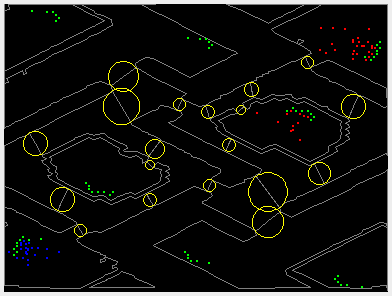
\includegraphics{graphics/environment-gui.png}
\caption{Our custom representation of the state of the environmen}
\label{fig:environment-gui}
\end{figure}

\section{Detectors}
\label{sec:detectors}
Feature detectors is how LIDA perceives it's environment and identifies important aspects of the current game state. They are task that are run at specific intervals and parses the game state at that time in order to identify a given feature that can later be used in different modules in LIDA recognize thoughts and concepts. Each detector usually only identifies one specific feature, but it is possible for one detector to identify several features of they are of the same type. 

These are the detectors we implemented: 
\begin{itemize}
\item \textbf{IdleWorkerFeatureDetector} \\
This feature detector identifies worker units that doesn't have a job, a worker could be gathering resources, constructing buildings or scouting. But for efficiency it should be doing something at all times. 
\item \textbf{ResourceFeatureDetector} \\
This feature detector identifies what type of units and buildings that we currently have enough resources available to create. This can be buildings we can construct, units we can morph or upgrades that we can research. 
\item \textbf{SupplyBlockFeatureDetector} \\
This feature detector identifies when we are getting close to being supply blocked, that means that we can't build any more units because another supply-granting building/unit is created.
\item \textbf{UnsaturatedResourcesFeatureDetector} \\
This feature detector identifies whether or not our available resource nodes have are saturated with enough workers that are gathering them. This can be used to decide if we need to build more workers or not.
\item \textbf{BuildOrderFeatureDetector} \\
This feature detector identifies what type of building we want to construct for our next step in the planed build order. For our simple implementation it detects if we have more resource generation then unit production buildings, so we need to expand our capacity by adding new ones. 
\item \textbf{IdleProductionFeatureDetector} \\
This feature detector identifies when a production building is currently not training any units. In Starcraft being effective with the resources you have available is important, therefor not queuing units on a production building is important.
\item \textbf{StructureFeatureDetector} \\
This feature detector identifies the buildings we have already constructed. This is important to know because we might not want to build another of the same building, and for unit production it is important to know what kind of production buildings we have available. 
\item \textbf{TimingAttackFeatureDetector} \\
This feature detector identifies when it is time to attack the enemy. In our current implementation is a very simple detector that just waits until we have collected a substantial army of units and then activates to detect that it is now time to attack.
\end{itemize}

Feature detectors can be created that detect almost every aspect of the game, and they can be everything from simply detecting the existence of specific units or game elements to more complex detectors that detect army compositions or enemy tactics and strategies. The more of them you implement the more advanced concepts you can identify and that opens up more advanced strategies you can perform yourself. 

\section{Attention Module}
One of the main features of a cognitive system, and even of the human brain, is the ability to focus its consciousness or give attention to a subsection of world as it perceives it. This is what the {\em Attention module} is responsible for. It achieves this by running attention codelets that look for specific workspace content from the current situational model and them creates coalitions from this that is added to the global workspace where they will compete with other coalitions for consciousness.

The activation for a coalition is based both on the activation for the PAM nodes that it contains and the activation for the codelet it self that created it. 

We included a number of different attention codelets in our implementation to bring content to consciousness:
\begin{itemize}
\item \textbf{Idle worker codelet} \\
A simple codelet that makes a coalition with idle worker node. This codelet has a high activation in order to make sure has a big change of winning the competition for consciousness since you want workers to be doing a job at all times. 
\item \textbf{Build worker codelet} \\
This codelet look for 3 different situations that decides if a worker should be created. That we can afford to create the worker, that our resources are not saturated already and that the base building is not currently training any units. 
\item \textbf{Build supply codelet} \\
This is another simple but important codelet that has a high activation value. It looks for the situation where we are supply blocked, or getting close to being supply blocked, and we can afford to build a supply structure. It has a high activation level because getting supply blocked means you can't create any more units until another supply structure is finished building, that will be a lot of valuable time lost where no units is trained. 
\item \textbf{Build Order Codelet} \\
This is one of the more complex codelets, it looks for all the buildings that we can currently afford as well as all the buildings that we need to create according to the build order nodes. Combining these in a coalition allows the action selector later to decide what building should be created next. 
\item \textbf{Train Units Codelet} \\ 
This codelet is similar to the Build Order Codelet, except it looks for the units we can afford to train in addition to what unit production buildings we currently have available to use. 
\item \textbf{Strategy Codelet} \\
This codelet looks for any node that is a child from the strategy node. These defensive or offensive strategies during a game. But in our implementation we only have a simple strategy that is to attack with every army unit we have at the same time when we feel we have a sufficient army size.
\end{itemize}

\section{Action Execution}
\label{sec:actionexecution}
After LIDA has selected a focus of conciseness and an appropriate action has been selected from the behaviour net, the selected action must be executed. This gets execute by having the sensory-motor memory make calls to the environment class that functions as the interface between LIDA and JNI-BWAPI. 

These are the possible action that gets selected and executed in Jantu:
\begin{itemize}
\item \textbf{Mine minerals} \\
This actions takes a worker that is not currently performing a task and orders it to start mining minerals from an unsaturated mineral deposit.
\item \textbf{Build worker} \\
This action starts training a worker unit at the main building in the home base, the Nexus for Protoss. 
\item \textbf{Build supply} \\
This action constructs a building or unit that grants increased supply. This can be a building or a unit depending on the race. For Protoss it creates a structure called a pylon that grants more available maximum supply.  	
\item \textbf{Build gateway} \\
This action works in much the same way as {\em Build supply} except that it creates a production building called gateway. This building is used to warp in(train) army units. 
\item \textbf{Train zealot} \\
This action sets a zealot for training at an available gateway that is currently not training any other units. It is important that it doesn't queue it at a gateway that is already training another unit since it locks up resources and is inefficient. 
\item \textbf{Attack} \\ 
This action executes an attack on enemy units. It can be a very simple action like in our implementation where it just used every available army unit and attacks the enemy, or it could be more complex like using groups of units for different attacks. Also worth noting that if you are not using perfect information then you can only attack units that you have seen by scouting or being invaded. 
\end{itemize}

How the action is implemented in the sensory-memory is up to the developer, as long as it performs its given function. It can be really simple implementation or you could do something more complex, LIDA is there to decide what parts or game state to focus on, and to make the decision on what action to perform, not how that action is executed.

\section{Parameter tweaking}
Like any other partially sub-symbolic artificial intelligence system, parameter tweaking is very important and small changes in the parameters can completely change how the agent behaves and acts. In LIDA there are a lot of activation values and thresholds for when something is counted as activated. 

The feature detectors are the first instances where activation is important, when they discover something from the input they send activation to one or more nodes in PAM, and this activation level will decide how important the model thinks this piece of information is, but in addition to this, it will also have cascading effects on the system further down the line. When attention codelets compete about access to the global workspace and consciousness broadcast the activation of the nodes contained in the codelets context together with the initial activation value of the codelet itself makes up the total activation of the codelet. So if some of the nodes have low activation from the feature detectors the codelet that contains that node will also be judged to be not so important. 

Learning of base activation levels are part of the LIDA model but are not yet implemented in the current version of the framework. When some nodes have been important in the past this will make them more likely to activate in the future, and will have a big impact on the performance of the agent. 

Both feature detectors and codelets in the framework are implemented as processes that run at specified intervals, defined by the number of ticks between each time they are run. Changing how often a process is run will also impact the agent in not so predictable ways. If you do not detect the presence of some piece of information in time, you might decide on an action that is not the optimal way to handle the situation of you had all the information available to you. If the period between the execution of a feature detector is to long, you can end up with the related PAM node decaying below the threshold for activation between each time the detector is run, but if the detector was run at more regular intervals it would stay activated constantly because the node would receive excitation after each run of the detector. 

All the elements in the LIDA framework that has activation have different parameters for how this activation is received and decayed. Decay of elements are configured differently for different modules. In Declarative Memory elements decay at a very slow rate, if at all, while in PAM they decay during a very short period of time, usually just a few ticks long. The same options for configuration of excitation exists in the framework. 

To facilitate easy tweaking of parameters in LIDA most of them can and should be configurable from the XML definition of the agent. This makes changing and testing new values a lot easier then having to rewrite lines of code between runs. 
